\documentclass{article}
\setcounter{tocdepth}{4} %Required to insert paragraph in TOC
\setcounter{secnumdepth}{4} %Required to insert paragraph in TOC

\usepackage{graphicx} % Required for inserting images
\graphicspath{ {./img/} }

\usepackage{blindtext}
\usepackage{titlesec}
\usepackage[dvipsnames]{xcolor}
\usepackage{geometry}
\geometry{
	a4paper,
	total={170mm,257mm},
	left=25mm,
	top=20mm,
}

\usepackage{adjustbox}
\usepackage{amsmath}
\usepackage{amsthm}
\usepackage{amssymb}
\usepackage{cancel}
\usepackage{caption}
\usepackage{subcaption}
\usepackage{titlesec}
\usepackage{float}
\usepackage{enumitem}
\usepackage{hyperref}
\usepackage{makecell}
\usepackage{chronology}
\usepackage{cleveref}
\usepackage{fancyhdr}
\usepackage{mathabx}
\usepackage{mathrsfs}
\usepackage{subfiles} %best loaded last in preamble

\pagestyle{fancy}

\setcounter{secnumdepth}{4}

\newcommand{\foo}{\hspace{-2.3pt}$\bullet$ \hspace{5pt}}

\titleformat{\paragraph}
{\normalfont\normalsize\bfseries}{\theparagraph}{1em}{}
\titlespacing*{\paragraph}
{0pt}{3.25ex plus 1ex minus .2ex}{1.5ex plus .2ex}

\newtheorem{definition}{Definizione}[section]
\newtheorem{theorem}{Teorema}[section]
\newtheorem{exmp}{Esempio}[section]

\numberwithin{equation}{subsection}

\title{Appunti Elettronica}
\author{Mattia Robuschi Caprara}
\date{}

\definecolor{CoverGreen}{RGB}{11, 112, 0}

\begin{document}

	\begin{titlepage}
		
		\pagecolor{CoverGreen}
		
		\vspace{25 mm}
		\begin{center}
			\large
			{\color{white}\textbf{Mattia Robuschi Caprara}} 
		\end{center}
		
		\begin{center}
			\huge
			{\color{white}\textbf{Appunti Elettronica}}
		\end{center}
		
		\vspace{45 mm}
		
		\begin{figure}[h]
			\centering
			\adjustbox{cfbox=white 5pt 0cm}{\includegraphics[scale=0.3]{0.cover.jpg}}
			%\caption{Caption}
			\label{fig:cover}
		\end{figure}
		
		\thispagestyle{empty} 
	\end{titlepage}

	\newpage
	\pagecolor{white}
	\section*{Prefazione}
	Un riassunto di elettronica (1) (Professor. Paolo Ciampolini).\\
	Questi appunti sono stati realizzati principalmente dai contenuti degli agli appunti di Paolo Panciroli, detto ciò non voglio prendere alcun merito visto che sono solo una revisione/riorganizzazione.\\\\
	P.S. Ricordo che il simbolo $\propto$ significa "\textbf{proportional to}" quando lo si vede indica che due elementi sono proporzionali.
	\tableofcontents
	\newpage
	
	\section{Materiali Semiconduttori}
	\subfile{sections/semicond}
	
	\section{Giunzione \textit{pn}}
	\subfile{sections/pn}
	
	\section{Transistore a Giunzione Bipolare \textit{BJT}}
	\subfile{sections/giunz_bip}
	
	\section{Transistore MOSFET}
	\subfile{sections/mosfet}
	
	\section{Realizzazione dei transistori}
	\subsection{Introduzione}
	Abbiamo più volte sottolineato, nel corso della trattazione dei transistori MOSFET come gli aspetti produttivi incidano fortemente sulle possibilità di realizzare logiche sempre più veloci.\\\\
	In questa Appendice vedremo alcuni aspetti tecnologici circa la realizzazione dei transistori.
	\subsection{Il processo di fabbricazione}
	Per realizzare logiche CMOS abbiamo bisogno di materiali semiconduttori monocristallini.\\\\
	Tutto quanto nasce da un substrato di semiconduttore (tipicamente il silicio).\\
	Il silicio non può però essere il silicio della sabbia o del vetro: per realizzare un transistore è necessario utilizzare un silicio estremamente puro e raffinato (la purezza deve essere paragonabile al drogaggio, cioè una parte per miliardo).\\
	Il raffinamento si ottiene solitamente tramite processi di fusione successivi.\\
	Alle temperature di fusione è però facile contaminare nuovamente il semiconduttore.\\\\
	Inoltre è necessario che il silicio presenti un reticolo cristallino molto ben definito.\\
	Questo è ottenibile immergendo in un bagno di silicio fuso un cristallo di silicio già formato che viene poi estratto con estrema lentezza.\\
	In questo modo è possibile creare un lingotto cristallino che viene successivamente affettato (in fette di circa mezzo millimetro) con mole diamntate.\\
	Lo spessore del dispositivo è “imposto” dalle lavorazioni meccaniche che richiedono una certa resistenza.\\\\
	Per via delle dimensioni richieste dal processo meccanico di creazione delle fette di semiconduttore, solamente una faccia è accessibile al progettista per la realizzazione del circuito integrato (Figura \ref{fig:im-232}).\\\\
	Tutte le procedure di raffinamento e cristallizzazione necessarie per portare al *grado elettronico* rendono il processo di creazione delle fette di silicio un processo molto lento e costoso tanto che solo poche aziende al mondo possono realizzare tali fette.
	\begin{center}
		\begin{figure}[h]
			\centering
			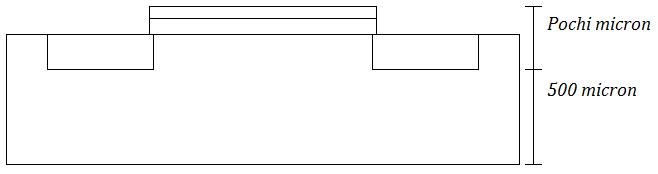
\includegraphics[scale=0.45]{232.png}
			\caption{La parte utilizzata per la realizzazione del circuito integrato è di pochi micron mentre il substrato è di circa 500 micron.}
			\label{fig:im-232}
		\end{figure}
	\end{center}
	\subsection{La realizzazione della struttura}
	Una volta ottenuta la fetta di silicio, essa viene lucidata per rimuovere le imperfezioni dovute al taglio con la sega diamantata ed ossidata.\\\\
	Le tasche con drogaggio differente sono tipicamente realizzate con processi fotolitografici.\\
	I principali sistemi per drogare il semiconduttore sono due.\\
	Il primo consiste nell'infornare ad elevata temperatura il silicio in forni la cui atmosfera sia satura di gas drogante.\\
	Il secondo (impiantazione ionica) consiste nello sparare ioni di drogante direttamente sulla fetta di silicio.\\
	Il primo metodo (a caldo) richiede svariati minuti mentre il secondo sistema (a freddo) rischia di danneggiare la superficie.\\\\
	Per evitare che vengano drogate anche zone che non devono essere drogate, si utilizzano alcuni strati di materiale "sacrificale" che verrà poi rimossa perché faccia da scudo alla fetta di silicio.\\
	Tipicamente prima si cresce uno strato di ossido di silicio sull'intera fetta e successivamente si distribuisce una certa quantità di gelatina fotosensibile (photoresist) sullo strato di silicio.\\
	Infine, utilizzando maschere di contatto o di proiezione si illuminano con raggi ultravioletti le zone che andranno ad essere drogate.\\
	Da ultimo è possibile rimuovere la parte esposta ai raggi ultravioletti.\\
	Una volta rimosso il photoresist dalle porzioni volute si inizia un nuovo attacco chimico (tipicamente con l'acido cloridrico) per erodere l'ossido.\\
	Eroso l'ossido dalle porzioni volute è possibile impiantare gli ioni droganti nelle zone non più protette dall'ossido.\\\\
	L'intero processo è molto lento.\\
	Questa lentezza è però comoda in quanto consente un controllo molto preciso del processo di produzione.
	\begin{center}
		\begin{figure}[h]
			\centering
			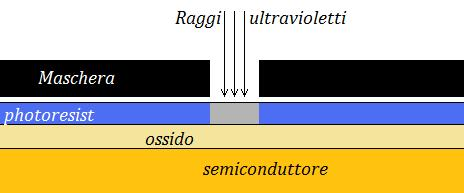
\includegraphics[scale=0.45]{233.png}
			\caption{Schema grafico del processo di creazione delle tasche.}
			\label{fig:im-233}
		\end{figure}
	\end{center}
	Il processo fotolitografico si può riassumere nei seguenti passi.
	\begin{enumerate}
		\item Definizione di una maschera.
		\item Cresicta dello scudo.
		\item Deposizione del photoresist.
		\item Impressione del photoresist.
		\item Attacco dell'ossido.
		\item Completamento della fase di produzione.
	\end{enumerate}
	Una volta effettuato il passo 6 si ricomincia dall'inizio per quante volte è necessario.
	\subsection{Problemi della realizzazione}
	La tecnologia attuale consente di realizzare questo tipo di strutture in pochi micron.\\
	Abbiamo però un problema: per definire l'immagine del transistore non possiamo usare una radiazione con lunghezza d'onda maggiore rispetto alle dimensioni del dispositivo.\\
	Per tale ragione, recentemente, si è passati dall'utilizzo dei raggi ultravioletti all'utilizzo dei raggi X e dei raggi elettronici (con conseguente aumento della complessità).\\\\
	Un secondo problema nella realizzazione dei circuiti integrati è che per inserire anche solo due dispositivi MOS è necessario ripetere per tre volte l'intero processo dalla creazione dello scudo fino al drogaggio.\\
	Allora il progettista non può che controllare le dimensioni in pianta del dispositivo.\\\\
	Un ulteriore problema consiste nell'allineamento delle maschere che deve essere perfetto.\\
	Se l'ossido non copre completamente e perfettamente il canale\\\\
	(tipicamente di pochi nanometri) il dispositivo non funziona.\\
	Questo problema è di facile soluzione grazie all'autoallineamento: prima si realizzeranno l'ossido ed il gate (tipicamente si utilizza il polisilicio poiché è più facile da gestire rispetto ai metalli) e poi si drogano le tasche laterali.
	\subsection{Realizzazione del circuito integrato}
	Abbiamo ora la necessità di realizzare il circuito vero e proprio necessario alla connessione di due transistori.\\
	Tipicamente questa fase consiste nello spargere un nitrato sull'intera superficie.\\
	Successivamente, con altri processi fotolitografici, si perfora lo strato isolante in corrispondenza delle tasche di drain e source.\\\\
	Successivamente si sparge una superficie metallica uniforme su tutto il dispositivo.\\
	Con un nuovo processo fotolitografico si realizzano infine le connessioni volute.
	\begin{center}
		\begin{figure}[h]
			\centering
			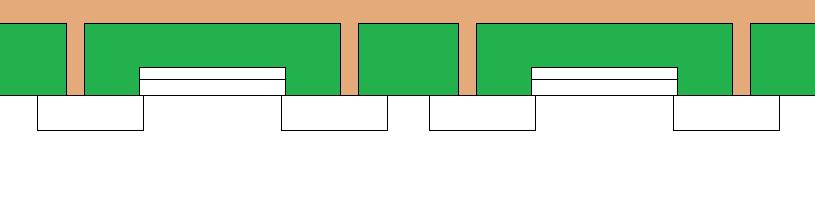
\includegraphics[scale=0.45]{234.png}
			\caption{Schema grafico della realizzazione delle interconnessioni. \\ In verde il nitrato; in color rame il metallo.}
			\label{fig:im-234}
		\end{figure}
	\end{center}
	Si presenta però di nuovo il problema dell'allineamento.\\
	In questo caso non possiamo però sfruttare l'autoallineamento.\\
	La soluzione consiste nell'utilizzo di una maschera un poco più grande rispetto alla maschera del gate in modo che, anche in caso di errore di allineamento, il circuito non entri in cortocircuito tra il drain ed il source.\\\\
	Un ennesimo problema consiste nella realizzazione delle interconnessioni: connettere due punti può richiedere di passare sopra a percorsi già realizzati.\\
	La soluzione consiste nell'utilizzare varie metalliazzazioni differenti (le tecnologie attuali hanno fino a dieci metallizzazioni).\\
	Ogni metallizzazione richiede però maschere opportune con le relative interconnessioni che sono attualmente la parte che occupa più spazione nella realizzazione di un circuito integrato.\\\\
	Attualmente si cerca di ridurre le dimensioni dei dispositivi assottigliando l'ossido e riducendo la lunghezza dei componenti.
	\subsection{Limiti dello sviluppo}
	Lo sviluppo di nuovi chip e circuiti integrati presenta alcuni limiti evidenti:
	\begin{enumerate}
		\item il costo di una macchina per la fotolitografia aumenta in modo esponenziale al diminuire delle dimensioni;
		\item mentre le tecnologie aumentano la propria produttività in modo esponenziale, i progettisti restano umani e richiedono sistemi CAD per poter progettare circuiti integrati sempre migliori;
		\item le potenze consumate dai chip aumentano in modo esponenziale;
		\item parimenti alle potenze consumate il calore dissipato aumenta in modo esponenziale;
		\item le dimensioni dello strato di ossido non possono essere ridotte a meno di uno strato atomico a meno di non trovare soluzioni alternative.
	\end{enumerate}
	
	\section{Esempi}
	\subsection{Esempio 1}
	Ricordando il modello a soglia del BJT:
	$$\text{Regione di interdizione} = \begin{cases} V_{BE} < V_{\gamma} \\ V_{CE} > V_{CESat} \\ I_B = 0 \\ I_C = 0 \end{cases} \quad V_{BC} < V'_{\gamma}$$
	$$\text{Regione normale} = \begin{cases} V_{BE} = V_{\gamma} \\ V_{CE} > V_{CESat} \\ I_B > 0 \\ I_C = \beta_F I_B \end{cases}$$
	$$\text{Regione di saturazione} = \begin{cases} V_{BE} = V_{\gamma} \\ V_{CE} = V_{CESat} \\ I_B = 0 \\ I_C < \beta_F I_B \end{cases}$$
	si ricavi la caratteristica ingresso-uscita del circuito di Figura \ref{fig:im-235}.
	\begin{center}
		\begin{figure}[h]
			\centering
			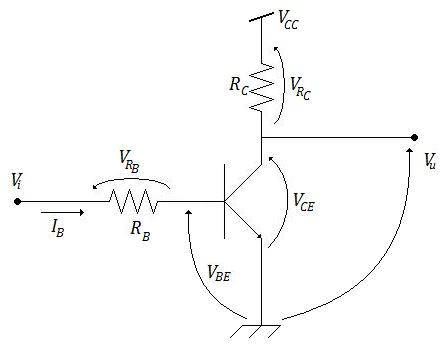
\includegraphics[scale=0.45]{235.png}
			\caption{Circuito in esame nell'Esempio 1.}
			\label{fig:im-235}
		\end{figure}
	\end{center}
	Il circuito è a vuoto: non abbiamo componenti connessi all'uscita.\\
	Allora sul ramo di uscita non circola corrente.\\\\
	Facciamo variare la tensione di ingresso nell'intervallo:
	$$0 \le V_i \le V_{CC}$$
	Il transistore è spento quando sia ha:
	$$V_{BE} < V_{\gamma}$$
	e quindi quando vale:
	$$V_i < V_\gamma$$
	dall'equazione alla maglia:
	$$V_i - V_{R_B} - V_{BE} = 0 \implies V_i = V_{R_B} + V_{BE}$$
	ricaviamo:
	$$V_{R_B} + V_{BE} < V_\gamma$$
	ed allora, per $V_i < V_\gamma$, il transistore non può che essere spento.\\
	Ma allora deve essere:
	$$I_C = I_B = I_E = 0$$
	$$V_{R_B} = 0$$
	$$V_i = V_{BE} < V_\gamma$$
	$$I_{R_C} = I_C = 0 \implies V_{R_C} = I_C R_C = 0$$
	e di conseguenza risulta:
	$$V_{CC} - V_{R_C} - V_{CC} = 0 \implies V_u = V_{CC}$$
	Dunque fino a che la tensione $V_i$ risulta inferiore a $V_\gamma$, la tensione di uscita è la tensione di alimentazione $V_{CC}$.\\\\
	Quando la tensione $V_{BE}$ raggiunge il valore di $V_\gamma$, il transistore si accende (usando il modello a soglia perdiamo la gradualità dell'accensione del transistore).\\
	Sul punto di transizione valgono sia le condizioni di transistore spento, sia le condizioni di transistore acceso.\\
	Il transistore si accende quando abbiamo:
	$$V_i = V_\gamma$$
	Ma, per quanto appena detto, avremo $V_u = V_{CC}$.\\
	Siccome però abbiamo anche $V_u = V_{CE}$ risulta essere $V_{CE} > V_{CESat}$ e dunque il transistore è in regione normale.\\\\
	Per $V_i > V_\gamma$ il transistore è sicuramente acceso.\\
	Siccome l'ingresso varia con continuità ipotizziamo di essere ancora in regione normale.\\
	Allora sarà:
	$$\begin{cases} V_{CC} - V_{R_C} - V_u = 0 \\ V_{R_C} = I_C R_C \\ I_C = \beta_F I_B \\ V_i - V_{R_B} - V_{BE} = 0 \\ V_{R_B} = R_B I_B \end{cases}$$
	da, sostituendo, cui ricaviamo:
	$$V_{CC} - \frac{\beta_F R_C}{R_B} (V_i - V_\gamma) - V_u = 0$$
	Allora, quando il transistore è in regione normale, risulta essere:
	$$V_u = \underbrace{V_{CC} + \frac{\beta_F R_C}{R_B} \cdot V_\gamma}_{\text{termine costante}} - \underbrace{\frac{\beta_F R_C}{R_B} \cdot V_i}_{\text{retta di uscita}}$$
	Questo risultato è valido fino a quando risulta essere $V_u > V_{CESat}$.\\
	Nel momento in cui si raggiunge $V_u = V_{CESat}$, il BJT entra in saturazione.\\
	In saturazione abbiamo:
	$$V_u = V_{CE} \Longrightarrow V_u = V_{CESat}$$
	Vogliamo però individuare il valore $V_i^*$ per cui l'uscita diviene $V_{CESat}$.\\
	Anche in questo caso sfruttiamo la transizione.\\
	Abbiamo il sistema:
	$$\begin{cases} V_u = V_{CC} + \frac{\beta_F R_C}{R_B} \cdot V_\gamma - \frac{\beta_F R_C}{R_B} \cdot V_i^* \\ V_u = V_{CESat} \end{cases}$$
	che, risolto, fornisce il valore cercato.\\\\
	La caratteristica ingresso-uscita del circuito in esame è riportata in Figura \ref{fig:im-236}.\\
	Si noti che il circuito è un invertitore e può essere usato per la realizzazione di una porta logica NOT.
	\begin{center}
		\begin{figure}[h]
			\centering
			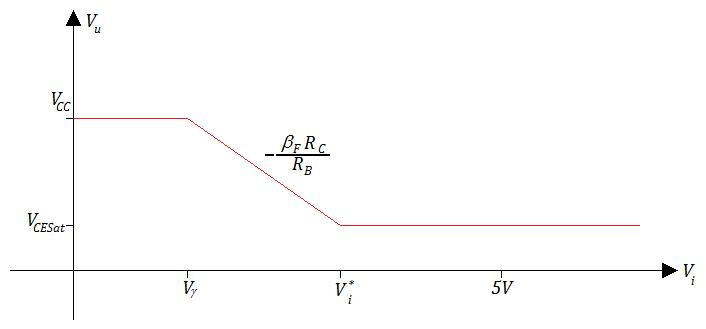
\includegraphics[scale=0.45]{236.png}
			\caption{Caratteristica ingresso-uscita del circuito nell'Esempio 1.}
			\label{fig:im-236}
		\end{figure}
	\end{center}
	\subsection{Esempio 2}
	Consideriamo ora il circuito di Figura \ref{fig:im-237} sapendo che è:
	$$\begin{cases} V_\gamma = 0,7 & V \\ 0 \le V_i \le 5 & V \\ R_1 = 4 & k\Omega \\ R_2 = 1 & k\Omega \\ R_3 = 500 & \Omega \\ \beta_F = 100 & \end{cases}$$
	\begin{center}
		\begin{figure}[h]
			\centering
			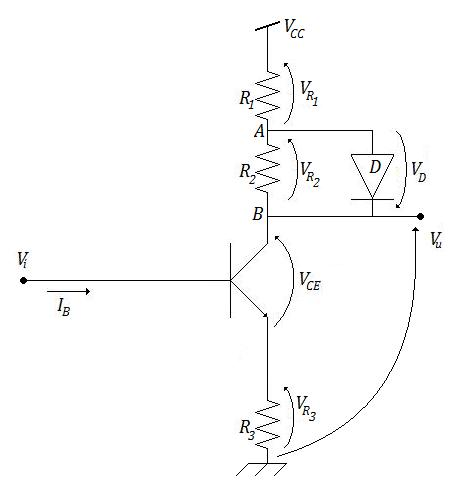
\includegraphics[scale=0.45]{237.png}
			\caption{Circuito in esame nell'Esempio 2.}
			\label{fig:im-237}
		\end{figure}
	\end{center}
	Quando il BJT è spento abbiamo:
	$$V_i < V_\gamma$$
	$$V_i - V_{BE} - R_3 I_3 = 0$$
	$$V_{BE} < V_\gamma$$
	$$I_E = I_B = I_C = 0$$
	$$V_u = V_{CC} - R_1 I_1 - R_2 I_2$$
	Se il diodo $D$ è acceso la corrente al nodo $A$ è:
	$$I_{R_1} = I_{R_2} + I_B$$
	mentra al nodo $B$ risulta:
	$$I_{R_2} + I_D = I_C$$
	ed allora è:
	$$I_{R_1} = I_C = 0 \implies I_{R_2} + I_D = 0 \implies I_{R_3} = -I_D$$
	che è un risultato assurdo.\\
	Allora l'ipotesi è errata e dunque il diodo deve essere spento e quindi l'unico risultato accettabile è:
	$$\begin{cases} I_D = 0 \\ I_{R_2} = 0 \end{cases}$$
	Quindi otteniamo:
	$$V_u = V_{CC}$$
	Per $V_i = V_\gamma$ siamo nel punto di transizione ed abbiamo:
	$$V_{BE} = V_\gamma$$
	$$I_C = 0 \implies I_D = 0$$
	ed il diodo continua ad essere spento.\\\\
	Per $V_i > V_\gamma$ ci poniamo nella condizione in cui il BJT è in regione normale ed il diodo è ancora spento.\\
	In queste condizioni è:
	$$\begin{cases} V_u = V_{CC} - (R_1 + R_2) I_C \\ I_C = \beta_F I_B \\ V_i - V_{BE} - R_3 I_E = 0 \\ I_E = (\beta_F + 1) I_B \approx \beta_F I_B \end{cases}$$
	$$V_u = V_{CC} - (R_1 + R_2) \cdot \beta_F \cdot \frac{V_i - V_\gamma}{R_3}$$
	$$V_u = 12 - 10V_i$$
	All'aumentare della tensione $V_i$ però si può raggiungere un punto in cui il diodo $D$ si accende.\\
	Potremmo però anche arrivare ad una condizione in cui il transistore entri in saturazione.\\\\
	La $V_i^*$ della saturazione del diodo è facilmente calcolabile imponendo $V_u = V_{CESat}$ nell'equazione appena ricavata per la $V_u$.\\
	Cerchiamo allora di trovare la $V_i^*$ nel caso in cui il transistore saturi.
	$$V_u = V_{CESat} - R_3 I_E$$
	$$V_i - V_\gamma - R_3 I_E = 0 \implies R_3 I_E = V_i - V_\gamma$$
	$$V_u = V_{CESat} + V_i - V_\gamma = -0,5 + V_i$$
	Per ricavare la minima $V_i^*$ mettiamo a sistema le tensioni di uscita nelle due diverse condizioni:
	$$\begin{cases} V_u = -0,5 + V_i \\ V_u = 12 + 10V_i \end{cases} \implies V_i^* = 1,136\ \text{V}$$
	Nel caso in cui si accenda il diodo è invece:
	$$V_{CC} - R_1 I_{R_1} - V_\gamma = V_u$$
	$$I_{R_1} = I_{R_2} + I_D = I_C \approx I_E$$
	$$V_i - V_\gamma - R_3 I_E = 0$$
	$$V_u = V_{CC} - R_1 I_C - V_\gamma = V_{CC} - R_1 \cdot \frac{V_i - V_\gamma}{R_3} - V_\gamma$$
	$$\begin{cases} V_u = -8V_i + 9,9 \\ V_u = 12 - 10V_i \end{cases} \implies V_i^* = 1,05\ \text{V}$$
	che è più piccola della precedente.\\
	Allora prima si accende il diodo e poi il transistore entra in saturazione.\\\\
	Il punto in cui il BJT entra in saturazione ed il diodo resta attivo troviamo:
	$$V_i^{**} = 1,15\ \text{V}$$
	Il grafico è riportato in Figura \ref{fig:im-238}.
	\begin{center}
		\begin{figure}[h]
			\centering
			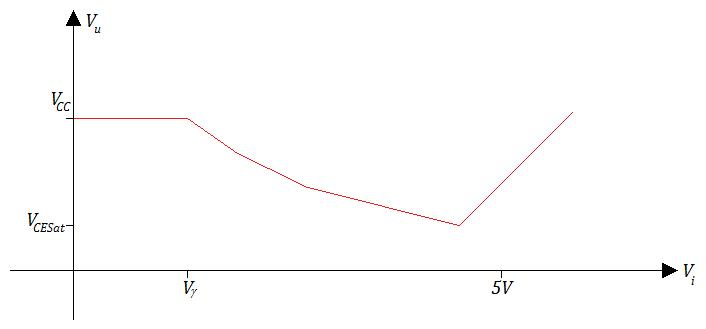
\includegraphics[scale=0.45]{238.png}
			\caption{Caratteristica ingresso-uscita del circuito nell'Esempio 2.}
			\label{fig:im-238}
		\end{figure}
	\end{center}
	
\end{document}